% ===========================================================================
% MONOGRAFIA COMPLETA
% Os capítulos 1 a 5 são os mesmos da parcial, revisados. O capítulo 6 (plano)
% sai; entram implementação, avaliação e conclusão.
% Compilar: latexmk final.tex   (ou: make final)
% ===========================================================================

\documentclass[12pt, openright, oneside, a4paper, english, brazil]{abntex2}

\newif\ifparcial
\parcialfalse

% ---------------------------------------------------------------------------
% Preâmbulo: pacotes e macros compartilhados por parcial.tex e final.tex
% Compilado com XeLaTeX (ver latexmkrc), por causa da fonte Arial.
% ---------------------------------------------------------------------------

% ---------------------------------------------------------------------------
% Fontes. O texto é Arial 12 (o tamanho vem da opção 12pt da classe). Numa
% máquina sem Arial instalada, usa-se a TeX Gyre Heros, clone livre da
% Helvetica, de métrica equivalente. A capa mantém a fonte serifada com que foi
% desenhada (TeX Gyre Termes, clone livre da Times).
% ---------------------------------------------------------------------------
\usepackage{amsmath}
\usepackage{fontspec}
\IfFontExistsTF{Arial}{%
  \setmainfont{Arial}
  \setsansfont{Arial}
}{%
  \setmainfont{texgyreheros}[Extension=.otf, UprightFont=*-regular,
    BoldFont=*-bold, ItalicFont=*-italic, BoldItalicFont=*-bolditalic]
  \setsansfont{texgyreheros}[Extension=.otf, UprightFont=*-regular,
    BoldFont=*-bold, ItalicFont=*-italic, BoldItalicFont=*-bolditalic]
}
\newfontfamily\fontecapa{texgyretermes}[Extension=.otf, UprightFont=*-regular,
  BoldFont=*-bold, ItalicFont=*-italic, BoldItalicFont=*-bolditalic]
% Letras e dígitos das poucas fórmulas do texto na mesma fonte do texto
\usepackage[italic]{mathastext}

\usepackage{indentfirst}
% Folga para parágrafos com fórmulas ou termos longos que não se quebram
\setlength{\emergencystretch}{2em}
\usepackage{microtype}
\usepackage{graphicx}
\usepackage{xcolor}
\usepackage{booktabs}
\usepackage{tabularx}
% Coluna de parágrafo alinhada à esquerda, para tabelas com texto (evita a
% hifenização forçada das colunas estreitas justificadas)
\newcolumntype{L}[1]{>{\raggedright\arraybackslash}p{#1}}
\usepackage{listings}
\usepackage{tikz}
\usetikzlibrary{positioning,arrows.meta,fit,backgrounds}

% Citações no padrão ABNT, autor-data
\usepackage[brazilian,hyperpageref]{backref}
\usepackage[alf]{abntex2cite}

\renewcommand{\backrefpagesname}{Citado na(s) página(s):~}
\renewcommand{\backref}{}
\renewcommand*{\backrefalt}[4]{%
  \ifcase #1 %
    Nenhuma citação no texto.%
  \or
    Citado na página #2.%
  \else
    Citado #1 vezes nas páginas #2.%
  \fi}

% ---------------------------------------------------------------------------
% Estética: fora da capa, tudo em preto. As duas cores abaixo são usadas
% apenas pela capa (config/capa.tex).
% ---------------------------------------------------------------------------
\definecolor{azulpoli}{HTML}{0B2A4A}
\definecolor{cinzacapa}{HTML}{5A6270}

\renewcommand{\ABNTEXchapterfont}{\bfseries}
\renewcommand{\ABNTEXsectionfont}{\bfseries}
\renewcommand{\ABNTEXsubsectionfont}{\bfseries}

\AtBeginDocument{%
  \hypersetup{
    pdftitle={\imprimirtitulo},
    pdfauthor={\autorumnome, \autordoisnome},
    pdfsubject={\imprimirtipotrabalho},
    hidelinks,
  }%
}

% Código C nas listagens: sem cor e sem negrito
\lstset{
  language=C,
  basicstyle=\ttfamily\small,
  keywordstyle=,
  commentstyle=\itshape,
  numbers=left,
  numberstyle=\tiny,
  frame=single,
  breaklines=true,
  showstringspaces=false,
}

% ---------------------------------------------------------------------------
% Marcação de trabalho pendente.
% Para a versão de entrega, troque \mostrarpendentestrue por \mostrarpendentesfalse:
% os marcadores somem do PDF sem precisar apagá-los do texto.
% ---------------------------------------------------------------------------
\newif\ifmostrarpendentes
\mostrarpendentesfalse
\newcommand{\pendente}[1]{%
  \ifmostrarpendentes{\color{red}[PENDENTE: #1]}\fi}

% Sem negrito no corpo do texto: os rótulos de listas de descrição (QP1, nomes
% das métricas) saem em estilo normal, seguidos de dois-pontos.
\renewcommand*{\descriptionlabel}[1]{\hspace{\labelsep}\normalfont #1:}

% Termos recorrentes
\newcommand{\isr}{\textit{ISR}}
\newcommand{\llm}{\textit{LLM}}

% ---------------------------------------------------------------------------
% Estilo visual do miolo: moderno e todo em preto. A capa (config/capa.tex)
% tem estilo próprio e não é afetada por este arquivo.
%
% A classe abntex2 é derivada da memoir, então os comandos abaixo são os da
% memoir (chapterstyle, pagestyle), aplicados por cima dos padrões da abntex2.
% ---------------------------------------------------------------------------

% --- Abertura de capítulo --------------------------------------------------
% Número grande e leve, título em negrito alinhado à esquerda, fio fino abaixo.
% Capítulos sem número (Resumo, Sumário, Referências) usam o mesmo título e fio.
\makechapterstyle{moderno}{%
  \renewcommand*{\chapterheadstart}{\vspace*{0pt}}
  \renewcommand*{\printchaptername}{}
  \renewcommand*{\chapternamenum}{}
  \renewcommand*{\chapnumfont}{\normalfont\fontsize{44}{44}\selectfont}
  \renewcommand*{\printchapternum}{\raggedright\chapnumfont\thechapter}
  \renewcommand*{\afterchapternum}{\par\nobreak\vskip 10pt}
  \renewcommand*{\printchapternonum}{}
  \renewcommand*{\chaptitlefont}{\normalfont\bfseries\fontsize{22}{27}\selectfont\raggedright}
  \renewcommand*{\printchaptertitle}[1]{%
    \chaptitlefont ##1\par\nobreak
    \vskip 10pt
    \hrule height 0.5pt\relax}
  \renewcommand*{\afterchaptertitle}{\par\nobreak\vskip 30pt}
}
\chapterstyle{moderno}

% --- Títulos de seção ---------------------------------------------------------
\renewcommand{\ABNTEXchapterfont}{\normalfont\bfseries}
\renewcommand{\ABNTEXsectionfont}{\normalfont\bfseries\fontsize{14}{17}\selectfont}
\renewcommand{\ABNTEXsubsectionfont}{\normalfont\bfseries}
\renewcommand{\ABNTEXsubsubsectionfont}{\normalfont\itshape}

% --- Cabeçalho ----------------------------------------------------------------
% Nome do capítulo à esquerda, página à direita, fio fino abaixo. Substitui o
% cabeçalho padrão da abntex2 (abntheadings) em todo o texto.
\makepagestyle{moderno}
\makeoddhead{moderno}{\small\leftmark}{}{\small\thepage}
\makeevenhead{moderno}{\small\leftmark}{}{\small\thepage}
\makeheadrule{moderno}{\textwidth}{0.4pt}
\makepsmarks{moderno}{%
  \createmark{chapter}{left}{shownumber}{}{\quad}
  \createplainmark{toc}{left}{\contentsname}
  \createplainmark{bib}{left}{\bibname}}
\aliaspagestyle{abntheadings}{moderno}

% --- Legendas, tabelas e código -------------------------------------------------
\captionnamefont{\small}
\captiontitlefont{\small}
\setlength{\heavyrulewidth}{0.6pt}
\setlength{\lightrulewidth}{0.3pt}
\lstset{frame=tb, framerule=0.4pt, framesep=6pt, xleftmargin=1.5em}

% ---------------------------------------------------------------------------
% Dados do trabalho, no formato do modelo do PCS: alimentam a capa e a folha
% de rosto geradas pela classe abntex2.
% ---------------------------------------------------------------------------

\titulo{Detecção de Defeitos de Concorrência em Software Embarcado Orientado a
Interrupções, com Triagem e Reparo Assistidos por Modelos de Linguagem}

\autor{Lucas de Oliveira Martim \\ Pedro Henrique Machado Almeida}

\local{São Paulo, SP}
\data{2026}

\orientador{Prof. Dr. Carlos Cugnasca}

\instituicao{%
  Universidade de São Paulo -- USP
  \par
  Escola Politécnica
  \par
  Departamento de Engenharia de Computação e Sistemas Digitais (PCS)}

\tipotrabalho{Monografia de Conclusão de curso (Graduação)}

\newcommand{\versaodocumento}{Trabalho de Conclusão de Curso}
% ---------------------------------------------------------------------------
% Capa: Escola Politécnica da USP, Engenharia de Computação
% Substitui a capa padrão do abntex2. O texto da versão (parcial ou completa)
% vem de \versaodocumento, definido em parcial.tex e final.tex.
% ---------------------------------------------------------------------------

% As cores azulpoli e cinzacapa vêm de config/preambulo.tex.

\renewcommand{\imprimircapa}{%
  \begin{capa}%
    \fontecapa
    \centering
    % --- Cabeçalho: selo da Poli, instituição, logotipo da USP ---
    \begin{minipage}[c]{0.2\textwidth}
      \centering
      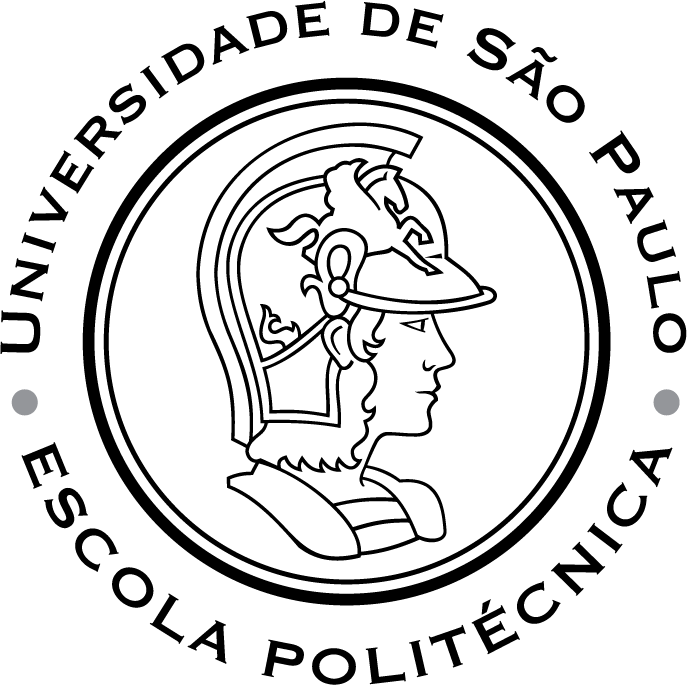
\includegraphics[height=2.9cm]{figuras/logo-poli}
    \end{minipage}%
    \hfill
    \begin{minipage}[c]{0.56\textwidth}
      \centering
      {\large\bfseries\MakeUppercase{Universidade de São Paulo}}\\[4pt]
      {\large\MakeUppercase{Escola Politécnica}}\\[8pt]
      {\small\color{cinzacapa}Departamento de Engenharia de Computação\\
       e Sistemas Digitais (PCS)}
    \end{minipage}%
    \hfill
    \begin{minipage}[c]{0.2\textwidth}
      \centering
      
\includegraphics[width=\linewidth]{figuras/logo-usp}
    \end{minipage}

    \vspace{0.6cm}
    {\color{azulpoli}\rule{\textwidth}{1.2pt}}

    \vfill

    % --- Título ---
    {\small\color{cinzacapa}\MakeUppercase{\curso}}\\[0.6cm]
    % 16,8 pt em vez do \LARGE (17,28 pt): no XeLaTeX não há expansão de fonte,
    % e o tamanho cheio quebrava o título em quatro linhas em vez de três.
    {\color{azulpoli}\fontsize{16.8}{22}\selectfont\bfseries\imprimirtitulo\par}
    \vspace{0.8cm}
    {\large\versaodocumento\par}

    \vfill

    % --- Autores ---
    \begin{tabular}{@{}l@{\hspace{1.2cm}}l@{}}
      \large\autorumnome   & \large\color{cinzacapa}NUSP \autorumnusp \\[6pt]
      \large\autordoisnome & \large\color{cinzacapa}NUSP \autordoisnusp
    \end{tabular}

    \vspace{1cm}
    {\normalsize Orientador: \imprimirorientador\par}

    \vfill

    {\color{azulpoli}\rule{\textwidth}{0.6pt}}\\[8pt]
    {\large\imprimirlocal\\[2pt] \imprimirdata\par}
  \end{capa}%
}


\preambulo{Trabalho de Conclusão de Curso apresentado à Escola Politécnica da
Universidade de São Paulo para obtenção do título de Engenheiro de Computação.}

\begin{document}

\selectlanguage{brazil}
\frenchspacing

\imprimircapa
\imprimirfolhaderosto*

\setlength{\absparsep}{18pt}
\begin{resumo}
Software embarcado orientado a interrupções está sujeito a \textit{data races} e
violações de atomicidade: uma rotina de tratamento de interrupção pode
interromper o código principal entre dois acessos a uma variável compartilhada
e corromper seu valor. As ferramentas da literatura priorizam a precisão, medem
mal o recall e tratam essas duas classes de defeito separadamente; apenas a mais
antiga propõe correções. Em paralelo, trabalhos recentes usam modelos de
linguagem para triar e reparar alertas de analisadores estáticos, mas todos
tratam defeitos sequenciais. Este trabalho propõe uma ferramenta que ocupa essa
interseção. Uma análise estática sobre a representação intermediária do LLVM
encontra os candidatos das duas classes sem falsos negativos, em relação a uma
lista explícita de premissas; um solver SMT descarta apenas o que prova
impossível; e um modelo de linguagem ordena, explica e propõe correções para os
candidatos restantes, sem nunca descartá-los. A avaliação usa o benchmark
Racebench, com gabarito recontado e corrigido (48 defeitos e 38 armadilhas),
métricas que não podem ser melhoradas descartando candidatos (portão de recall,
rejeição de armadilhas e \textit{Inspection Ratio}) e uma ablação das técnicas de
\textit{prompt}. Esta monografia parcial apresenta a fundamentação, a revisão da
literatura, a proposta, a metodologia de avaliação e o cronograma do trabalho.

Palavras-chave: concorrência. interrupções. software embarcado.
análise estática. modelos de linguagem.
\end{resumo}

\begin{resumo}[Abstract]
\begin{otherlanguage*}{english}
Interrupt-driven embedded software suffers from concurrency defects where an interrupt service routine may fire between two
accesses to a shared variable and corrupt its value. Existing tools favour
precision, measure recall poorly, and only the oldest one proposes fixes.
Meanwhile, recent work uses large language models to triage and repair
static-analyzer alerts, but all of it addresses sequential defects. This work
sits at the empty intersection between the two literatures. A static analysis
over LLVM's intermediate representation finds candidates with no false
negatives relative to an explicit list of assumptions, an SMT solver discards
only what it proves impossible, and a language model ranks, explains and
proposes fixes for the remaining candidates without ever discarding them. The
evaluation uses the Racebench benchmark with a recounted and corrected ground
truth, metrics that cannot be improved by discarding candidates, namely the
recall gate, trap rejection and the Inspection Ratio, and an ablation of prompt
techniques. This partial report presents the conceptual background, the work
method, the requirements, the tool design and the evaluation procedure.

\vspace{\onelineskip}

\noindent
\textbf{Keywords}: concurrency. interrupts. embedded software. static analysis.
large language models.
\end{otherlanguage*}
\end{resumo}

% Listas e sumário, na ordem do modelo do PCS.

\pdfbookmark[0]{\listfigurename}{lof}
\listoffigures*
\cleardoublepage

\pdfbookmark[0]{\listofquadrosname}{loq}
\listofquadros*
\cleardoublepage

\pdfbookmark[0]{\listtablename}{lot}
\listoftables*
\cleardoublepage

\begin{siglas}
  \item[BMC] \textit{Bounded Model Checking}, verificação de modelos limitada
  \item[CFG] \textit{Control-Flow Graph}, grafo de fluxo de controle
  \item[ISR] \textit{Interrupt Service Routine}, rotina de tratamento de interrupção
  \item[JSON] \textit{JavaScript Object Notation}, formato textual de dados estruturados
  \item[LLM] \textit{Large Language Model}, modelo de linguagem de grande escala
  \item[LLVM] infraestrutura de compiladores usada pela análise estática
  \item[SAT] \textit{Boolean Satisfiability}, satisfazibilidade booleana
  \item[SMT] \textit{Satisfiability Modulo Theories}
  \item[SVF] \textit{Static Value-Flow}, framework de análise de ponteiros sobre LLVM
\end{siglas}

\pdfbookmark[0]{\contentsname}{toc}
\tableofcontents*
\cleardoublepage


\textual

\chapter{Introdução}
\label{cap:introducao}

% Fontes no wiki: Thesis Goal, Synthesis, LLM Integration Patterns.

\section{Contexto}
\label{sec:contexto}

Sistemas embarcados de missão crítica, como controle aeroespacial, frenagem automotiva e \textit{drivers} de dispositivos, reagem ao hardware por meio de
interrupções. Quando um periférico sinaliza um evento, o processador suspende o
código em execução e desvia para uma rotina de tratamento de interrupção
(\textit{Interrupt Service Routine}, \isr). Ao término da rotina, a execução
retorna ao ponto em que foi interrompida.

Esse mecanismo introduz concorrência mesmo em programas sem \textit{threads}:
uma \isr\ pode ser disparada entre duas instruções quaisquer do código
principal, e ambos podem ler e escrever as mesmas variáveis globais. Se o
programador não proteger essas variáveis, o resultado do programa passa a
depender do instante exato em que a interrupção ocorreu.
\citeonline{sdracer} relatam um caso concreto em uma versão do uCLinux, em que
um \textit{driver} serial e um tratador de interrupção compartilham a linha de
comunicação e, num caminho de execução raro, transmitem dados
simultaneamente.

\section{O problema}
\label{sec:problema}

Este trabalho trata de duas classes de defeito de concorrência em programas
orientados a interrupções. Um \textit{data race} ocorre quando dois acessos à
mesma posição de memória, em fluxos diferentes e sendo ao menos um deles uma
escrita, podem acontecer sem ordem definida entre si. Uma violação de
atomicidade ocorre quando dois acessos de um mesmo fluxo, que o programador
supunha indivisíveis, são separados por um acesso de uma \isr\ à mesma
variável, de modo que o resultado não corresponde a nenhuma execução em
sequência. Os dois conceitos são definidos com precisão no
Capítulo~\ref{cap:fundamentacao}.

Esses defeitos são difíceis de detectar, isolar e corrigir, porque dependem da intercalação das execuções \cite{sdracer}: uma interrupção precisa chegar num intervalo de poucas instruções, e uma bateria de testes pode passar em todas as execuções observadas sem nunca exercitar esse intervalo. Por isso a literatura recorre a técnicas que raciocinam
sobre todas as execuções possíveis: análise estática, execução simbólica e
verificação de modelos.

\section{A lacuna}
\label{sec:lacuna}

A revisão da literatura (Capítulo~\ref{cap:relacionados}) identifica três
lacunas que motivam este trabalho.

As ferramentas priorizam precisão e medem mal o recall. Três das quatro
ferramentas estudadas relatam zero ou quase zero falsos positivos nos próprios
benchmarks, enquanto a ausência de falsos negativos é afirmada por inspeção
manual ou dentro de um limite de desenrolamento
\cite{sdracer,intrace,nichecker}. \citeonline{bmc4av} afirmam que uma ferramenta
com 100\% de precisão encontrou apenas 39,4\% das violações existentes na mesma
suíte. Como se discute na Seção~\ref{sec:rel-comparacao}, essa afirmação depende também de como os defeitos são contados. Essa cultura de avaliação tem
origem identificável: o benchmark que todos usam foi criado para uma
competição que, nos casos simples, penalizava um falso positivo em 3 pontos e premiava uma
detecção com apenas 2 \cite{racebench}.

Nenhuma ferramenta trata as duas classes de defeito, e só a mais antiga
repara. As ferramentas de \textit{data race} e as de violação de atomicidade
formam linhas separadas, e apenas o SDRacer, de 2020, propõe correções
\cite{sdracer}.

Modelos de linguagem já ajudam a análise estática, mas nunca em
concorrência. Trabalhos recentes usam modelos de linguagem de grande escala
(\llm) para decidir quais alertas de um analisador são reais
\cite{llift,chatgpt-static,reducing-fp}, inferir especificações
\cite{iris,adataint} e propor correções \cite{skipanalyzer,sastgenius}. Todos
tratam defeitos sequenciais: fluxo de dados contaminados, desreferência de
ponteiro nulo, vazamento de recursos, uso antes da inicialização.
\citeonline{llift} citam explicitamente a concorrência como algo que a análise
estática modela mal, sem tratá-la. A interseção entre as duas literaturas está
vazia, e é nela que este trabalho se situa.

\section{Objetivos}
\label{sec:objetivos}

\subsection{Objetivo geral}

Construir uma ferramenta que encontre \textit{data races} e violações de
atomicidade em código C embarcado orientado a interrupções sem falsos
negativos em relação a um conjunto explícito de premissas, aceitando falsos
positivos, e que feche o ciclo com um modelo de linguagem: detectar,
contextualizar, triar, reparar e re-verificar.

\subsection{Objetivos específicos}

\begin{enumerate}
  \item Detectar, numa única análise estática, os candidatos das duas classes de
    defeito, com recall de 100\% sobre o gabarito do Racebench.
  \item Emitir, para cada candidato, um registro de contexto com as evidências de
    que um revisor precisa: acessos, fluxos, prioridades, caminhos de chamada e
    estado de mascaramento.
  \item Descartar apenas candidatos que um solver prove impossíveis.
  \item Usar um \llm\ para ordenar e explicar os candidatos restantes, reduzindo
    o esforço de revisão sem nunca descartar um candidato.
  \item Medir a contribuição de cada técnica de \textit{prompt}, numa ablação no
    formato de \citeonline{llift}.
  \item Propor correções específicas de interrupção e verificar que o defeito
    desapareceu sem introduzir outros.
\end{enumerate}

\section{Justificativa}
\label{sec:justificativa}

Do ponto de vista prático, um defeito de concorrência que escapa aos testes se manifesta em campo, num sistema de controle físico. Uma análise que não perde defeitos é o que permite
afirmar que um programa foi verificado. O preço dessa garantia são os falsos
alarmes: na ferramenta IntRace, a primeira etapa gera cerca de 208 candidatos
por programa real \cite{intrace}. Revisá-los um a um é caro. A etapa com \llm\
proposta aqui ataca exatamente esse custo, ordenando os candidatos de modo que
o revisor encontre os defeitos reais lendo o mínimo possível, sem que nenhum
defeito saia do relatório.

Do ponto de vista científico, o trabalho contribui em três frentes: é a
primeira aplicação de triagem por \llm\ a concorrência com interrupções; unifica
num só \textit{front end} as duas classes de defeito que a literatura trata
separadamente; e explicita as premissas sob as quais a ausência de falsos
negativos vale, o que nenhum dos trabalhos revisados faz.

\section{Organização do documento}
\label{sec:organizacao}

O Capítulo~\ref{cap:fundamentacao} apresenta os conceitos necessários:
interrupções, as duas classes de defeito, as técnicas de análise e as métricas
de avaliação. O Capítulo~\ref{cap:relacionados} apresenta e compara os
trabalhos relacionados nas duas literaturas. O Capítulo~\ref{cap:proposta}
descreve a ferramenta proposta, e o Capítulo~\ref{cap:metodologia}, como ela
será avaliada.
\ifparcial
O Capítulo~\ref{cap:plano} apresenta o plano de trabalho.
\else
Os Capítulos~\ref{cap:implementacao}, \ref{cap:avaliacao} e
\ref{cap:conclusao} apresentam a implementação, a avaliação e as conclusões. O
Apêndice~\ref{ap:contratos} detalha os contratos de dados entre as etapas da
ferramenta.
\fi

\chapter{Fundamentação teórica}
\label{cap:fundamentacao}

Este capítulo apresenta os conceitos sobre os quais o restante do trabalho se
apoia. A Seção~\ref{sec:interrupcoes} descreve o modelo de execução de
programas orientados a interrupções; a Seção~\ref{sec:defeitos}, os defeitos
que se busca encontrar; a Seção~\ref{sec:tecnicas}, as técnicas de análise
usadas pela literatura e por este trabalho; a Seção~\ref{sec:soundness}, como
se mede a qualidade de um detector; e a Seção~\ref{sec:llm}, o que são os
modelos de linguagem e como são usados na análise de programas.

\section{Programas orientados a interrupções}
\label{sec:interrupcoes}

% wiki: concepts/Asymmetric Preemption, Interrupt Nesting,
%       Interrupt Masking and Synchronization

\subsection{Interrupções, ISRs e prioridades}

Um programa orientado a interrupções é formado por um fluxo principal
(\textit{main}), que executa continuamente, e por um conjunto de rotinas de
tratamento de interrupção. Formalmente, a literatura o descreve como
$P = \mathit{Main} \parallel \mathit{ISR}_1 \parallel \dots \parallel
\mathit{ISR}_n$, com uma função que atribui uma prioridade a cada fluxo
\cite{bmc4av}. Cada fluxo é uma raiz de execução: tudo o que ele alcança por
chamadas de função pode ser executado sob sua identidade.

Uma \isr\ pode interromper (\textit{preemptar}) o fluxo principal, e uma \isr\
de prioridade maior pode interromper outra de prioridade menor. A convenção de
numeração varia na literatura: \citeonline{sdracer} e \citeonline{intrace}
formalizam números maiores como prioridades menores, enquanto
\citeonline{bmc4av} adotam o contrário. O benchmark usado por todos esses
trabalhos declara explicitamente que número maior significa prioridade
maior \cite{racebench}, e essa é a convenção adotada aqui.

\subsection{Preempção assimétrica}

A preempção entre interrupções é assimétrica: uma \isr\ interrompe o
fluxo principal, mas o fluxo principal nunca interrompe uma \isr; uma \isr\ de
alta prioridade interrompe uma de baixa, e nunca o contrário. Entre
\textit{threads}, ao contrário, a preempção é simétrica.

\citeonline{sdracer} tiram daí três consequências. Primeiro, uma \isr\ não pode
bloquear: ela executa até o fim, a menos que outra de prioridade maior a
interrompa. Segundo, a relação \textit{happens-before}, base da detecção de
condições de corrida entre \textit{threads}, deixa de ser correta quando uma
interrupção ocorre durante o cálculo dela. Terceiro, a sincronização não é
feita com travas (\textit{locks}), mas com mascaramento de interrupções. Por
isso as técnicas de \textit{threads} não se transferem diretamente, e a
literatura sobre interrupções recorre a padrões de acesso e a prioridades.

\subsection{Aninhamento}

Uma \isr\ interrompida por outra de prioridade maior, que por sua vez pode ser
interrompida, forma uma cadeia de aninhamento
(\textit{nesting}). O aninhamento multiplica as intercalações possíveis e é a
característica que mais separa as ferramentas: o NIChecker o trata
nativamente, o IntRace por uma conversão sequencial de dentro para fora, e o
SDRacer exclui explicitamente interrupções reentrantes
\cite{nichecker,intrace,sdracer}.

\subsection{Sincronização por mascaramento}

Como não há travas, o programador impede a interrupção de ocorrer:
mascara a interrupção antes de um trecho crítico e a reabilita depois.
No benchmark Racebench, isso é feito com \texttt{disable\_isr(n)} e
\texttt{enable\_isr(n)}, em que \texttt{n = -1} significa todas as
interrupções \cite{racebench}. Em código real, o mascaramento pode vir de APIs
padronizadas (como \texttt{disable\_irq} no Linux), de escritas diretas em
registradores ou de variáveis de controle, e \citeonline{intrace} pedem ao
usuário um arquivo de configuração que liste esses mecanismos não padronizados.

Dois cuidados decidem se uma análise de mascaramento perde defeitos. O
primeiro: uma interrupção só pode ser considerada mascarada num ponto se
estiver mascarada em todos os caminhos que chegam a esse ponto;
``mascarada em algum caminho'' não basta. O segundo, menos evidente: o
mascaramento feito por um fluxo pode ser desfeito por outro. No caso
\texttt{svp\_simple\_001\_001} do Racebench, o fluxo principal mascara a
interrupção 2 durante todo o intervalo de um defeito anotado; ainda assim o
defeito é real, porque a interrupção 1 continua habilitada, interrompe esse
intervalo e reabilita a interrupção 2 por dentro. Uma análise que olhe só para
o fluxo principal descartaria um defeito real.

\section{Defeitos de concorrência}
\label{sec:defeitos}

% wiki: concepts/Data Race, Atomicity Violation, Access Interleaving Patterns,
%       Pair-Triple Unification

\subsection{Data race}

Em programas com interrupções, um \textit{data race} é definido em termos de
preempção, e não de simultaneidade. \citeonline{intrace} o descrevem como dois
eventos de fluxos diferentes que acessam o mesmo objeto, sendo ao menos um
deles uma escrita, e em que o evento que interrompe tem prioridade maior.
\citeonline{sdracer} acrescentam uma condição de hardware: a interrupção que
interrompe precisa estar habilitada no instante do primeiro acesso. O defeito
envolve dois acessos e é uma pergunta sobre um instante: a
rotina $B$ pode executar exatamente no ponto do acesso $A$?

\subsection{Violação de atomicidade}

Uma violação de atomicidade envolve três acessos à mesma variável: dois
do fluxo interrompido, $A_1$ e $A_2$, e um acesso $B$ de uma \isr\ que ocorre
entre eles. O defeito existe quando a execução resultante não equivale a
nenhuma execução em série dos fluxos (atomicidade como serializabilidade).
Diferentemente do \textit{data race}, é uma pergunta sobre um
intervalo: $B$ pode executar em algum ponto de $[A_1, A_2]$?

Das oito combinações de leitura (R) e escrita (W) sobre a tripla, quatro não são
serializáveis e constituem violações. A Tabela~\ref{tab:padroes} mostra cada
uma e por que ela quebra a atomicidade.

\begin{table}[htb]
  \centering
  \caption{Os quatro padrões de violação de atomicidade}
  \label{tab:padroes}
  \begin{tabular}{@{}lL{10cm}@{}}
    \toprule
    Padrão $(A_1, B, A_2)$ & Por que quebra a atomicidade \\
    \midrule
    $(R,W,R)$ & as duas leituras do mesmo fluxo veem valores diferentes \\
    $(R,W,W)$ & $A_2$ escreve com base numa leitura que ficou obsoleta \\
    $(W,R,W)$ & a \isr\ enxerga um valor intermediário que não deveria existir \\
    $(W,W,R)$ & $A_2$ lê o valor escrito pela \isr, e não o escrito por $A_1$ \\
    \bottomrule
  \end{tabular}
  \fonte{Elaborada pelos autores.}
\end{table}

As outras quatro combinações, $(R,R,\ast)$, $(W,R,R)$ e $(W,W,W)$, são
serializáveis e não constituem violação. O padrão $(R,W,W)$ é disputado na
literatura: \citeonline{bmc4av} o classificam como benigno e o excluem, enquanto
\citeonline{nichecker} o contam como defeito. Este trabalho o mantém, porque o
gabarito do Racebench o anota em 10 dos 48 defeitos
(Seção~\ref{sec:rel-benchmarks}).

\subsection{A relação entre as duas classes}

Toda violação de atomicidade $(A_1, B, A_2)$ se projeta em dois pares
adjacentes, $(A_1, B)$ e $(B, A_2)$. Nos quatro padrões da
Tabela~\ref{tab:padroes}, cada um desses pares contém ao menos uma escrita, e
portanto é um \textit{data race} em potencial. Assim, na etapa de casamento de
padrões, o conjunto de pares contém o conjunto de triplas. Essa contenção foi
verificada nos 48 defeitos anotados do Racebench, sem exceção.

A contenção, porém, não sobrevive a um filtro de mascaramento. Considere o
trecho da Listagem~\ref{lst:secoes}, em que cada acesso do fluxo principal está
protegido por sua própria seção crítica, mas o intervalo entre elas não está.

\begin{lstlisting}[caption={Violação de atomicidade sem \textit{data race}},label={lst:secoes}]
void task(void) {
    disable_isr(1);  a = shared;     enable_isr(1);  /* A1 */
    /* ... interrupcoes habilitadas aqui ... */
    disable_isr(1);  shared = a + 1; enable_isr(1);  /* A2 */
}
void isr_1(void) { shared = 0; }                     /* B  */
\end{lstlisting}

Não há \textit{data race}: $B$ não pode ocorrer no instante de $A_1$ nem no de
$A_2$. Mas $B$ pode ocorrer entre as duas seções críticas, o que é uma violação
de atomicidade real. Um detector que trabalhasse só com pares, com um filtro de
mascaramento correto, não reportaria nada aqui. A conclusão, que orienta a
proposta do Capítulo~\ref{cap:proposta}, é que as duas classes podem
compartilhar a enumeração de acessos, mas devem ser derivadas e filtradas
separadamente.

\subsection{Defeito nocivo e defeito benigno}

Nem todo defeito tem consequência. \citeonline{intrace} adotam o critério de
Bai et al.: um \textit{data race} é nocivo se a variável compartilhada alimenta
uma condição de desvio (\texttt{if}, \texttt{while}) ou é usada como índice de
vetor ou ponteiro. Os mesmos autores apontam condições de corrida
deliberadamente deixadas sem proteção, por razões de tempo real, como uma
fonte de seus falsos positivos. A nocividade é, portanto, um julgamento sobre a
intenção do programa, distinto da pergunta sobre se a intercalação é possível.

\section{Técnicas de análise de programas}
\label{sec:tecnicas}

% wiki: concepts/Symbolic Execution, Bounded Model Checking,
%       Lazy Sequentialization, Loop Abstraction, Path Feasibility Analysis

\subsection{Análise estática}

A análise estática raciocina sobre o código sem executá-lo. Três estruturas são
centrais aqui. O grafo de chamadas indica quais funções cada função
pode chamar e, com isso, tudo o que é alcançável a partir de cada fluxo. O
grafo de fluxo de controle (CFG) indica, dentro de uma função, em que
ordem as instruções podem executar. A análise de ponteiros indica a
que posições de memória cada ponteiro pode apontar; ela é do tipo
\textit{may} (``pode apontar'') quando superaproxima as possibilidades, e do
tipo \textit{must} (``certamente aponta'') quando as subaproxima. Para não perder
defeitos, é preciso usar a forma \textit{may}: uma posição é compartilhada
quando os conjuntos de posições que dois fluxos podem acessar se interceptam.

Este trabalho faz a análise sobre a representação intermediária do compilador
LLVM \cite{llvm} e usa a biblioteca SVF para a análise de ponteiros
\cite{svf}. Os metadados de depuração do LLVM (\texttt{DILocation}) permitem
associar cada instrução analisada a uma linha do código-fonte C, o que é
indispensável para que um revisor, humano ou modelo de linguagem, consiga
entender o resultado.

\subsection{Execução simbólica}

Na execução simbólica, as entradas do programa são tratadas como símbolos, e
cada caminho percorrido acumula uma condição sobre esses símbolos. Um solver
decide se a condição é satisfazível, isto é, se existe alguma entrada que leve
o programa por aquele caminho. \citeonline{sdracer} usam a técnica para gerar
entradas e intercalações de interrupções que alcancem os pontos suspeitos, e
observam que registradores de hardware não são variáveis livres: seus valores
dependem do modelo do dispositivo.

\subsection{Verificação de modelos limitada}

A verificação de modelos limitada (\textit{Bounded Model Checking}, BMC)
procura defeitos em todas as execuções de comprimento até um limite $u$,
codificando o programa como uma fórmula para um solver SAT ou SMT. Sua
vantagem é produzir um contraexemplo, isto é, uma execução concreta que
exibe o defeito. Sua limitação é que o espaço de estados cresce
exponencialmente com $u$: alguns casos do Racebench exigem desenrolar um laço
10.000 vezes antes de o defeito aparecer \cite{nichecker}. A ferramenta de
referência dessa família é o CBMC \cite{cbmc}.

Duas técnicas atenuam o problema. A sequencialização preguiçosa
(\textit{lazy sequentialization}) traduz o programa concorrente num programa
sequencial não determinístico que simula suas execuções, e o entrega a um
verificador sequencial \cite{lazycseq}. A abstração de laços substitui
laços por versões superaproximadas antes do desenrolamento, para que defeitos
profundos apareçam com um limite pequeno \cite{nichecker}. Em qualquer caso,
um resultado ``sem contraexemplo'' vale apenas até o limite escolhido; não é
uma prova de ausência de defeitos.

\subsection{Viabilidade de caminho com solver SMT}

A análise de viabilidade de caminho decide se alguma execução real alcança os
acessos de um candidato na ordem exigida. \citeonline{intrace} constroem um
resumo simbólico da \isr, inserem o bloco de alta prioridade no bloco de baixa
prioridade no ponto de preempção e entregam as restrições de caminho ao solver
Z3 \cite{z3}. Se o solver responde que as restrições são insatisfazíveis
(\textit{UNSAT}), a intercalação é impossível, e isso é uma prova.
Essa propriedade é central neste trabalho: só uma prova de impossibilidade, como essa, autoriza descartar um candidato.

\section{Soundness, recall e precisão}
\label{sec:soundness}

% wiki: concepts/Soundness and False Negatives, Precision Metrics

Um falso positivo é um alerta que não corresponde a um defeito real;
um falso negativo é um defeito real que não gerou alerta. Uma análise é
\textit{sound} (correta) em relação a um conjunto de premissas quando não
produz falsos negativos sob essas premissas. A ausência incondicional de falsos
negativos não é alcançável para C com ponteiros, tabelas de vetores de
interrupção e fluxo de controle dependente de hardware; o que se pode afirmar
honestamente é a ausência relativa a uma lista explícita de premissas.

A Tabela~\ref{tab:metricas} resume as métricas usadas na literatura e neste
trabalho.

\begin{table}[htb]
  \centering
  \caption{Métricas de avaliação}
  \label{tab:metricas}
  \begin{tabular}{@{}L{3.6cm}L{5.4cm}L{5.0cm}@{}}
    \toprule
    Métrica & Definição & O que responde \\
    \midrule
    Precisão & $TP / (TP + FP)$ & quanto do que foi reportado é real \\
    Recall (taxa de acerto) & $TP / (TP + FN)$ & quanto do que existe foi encontrado \\
    \textit{Inspection Ratio} & $(TP + FP) / (TP + FP + TN + FN)$ & quanto é preciso ler \\
    \bottomrule
  \end{tabular}
  \fonte{\citeonline{reducing-fp}; elaborada pelos autores.}
\end{table}

Este trabalho prioriza o recall, e a razão é concreta: uma ferramenta pode ter
precisão perfeita examinando apenas o que o usuário indicou e, ainda assim,
perder a maioria dos defeitos. A precisão, sozinha, pode ser melhorada
descartando candidatos; o \textit{Inspection Ratio} não, pois mede a fração do
conjunto que um revisor precisa ler até encontrar todos os defeitos reais. Com
o recall mantido em 100\% por construção, é o \textit{Inspection Ratio} que
mostra o custo da ferramenta \cite{reducing-fp}.

\section{Modelos de linguagem na análise de programas}
\label{sec:llm}

% wiki: concepts/Prompt Architecture, LLM Triage

Um modelo de linguagem de grande escala (\llm) é uma rede neural treinada para
continuar textos, capaz de ler e produzir código. A instrução dada a ele é
chamada de \textit{prompt}. Para uso por outro programa, pede-se ao modelo uma
saída estruturada, isto é, uma resposta num formato fixo como JSON,
que possa ser lida e validada automaticamente.

Três limitações importam para este trabalho. Um \llm\ pode alucinar,
afirmando com confiança fatos falsos sobre o código. Suas respostas
variam entre execuções, de modo que uma mesma pergunta pode receber
veredictos diferentes. E seu uso tem custo, medido em
\textit{tokens}: \citeonline{llift} relatam cerca de 7.000 \textit{tokens}
e US\$~0,43 por candidato analisado, com o GPT-4 e os preços de 2024.

A literatura mostra que a forma como a interação é estruturada pesa mais que o
modelo escolhido. Na ablação de \citeonline{llift}, o mesmo modelo, sobre os
mesmos dados, passa de um recall de 0,15 com uma pergunta direta para 1,00 com
quatro componentes: ensino de uma regra do domínio por exemplos, pedidos
progressivos de contexto (o modelo pede as definições de que precisa),
decomposição da tarefa em conversas separadas e autovalidação contra regras
enviesadas para o lado seguro. Esses componentes são a base do desenho da
etapa de \llm\ deste trabalho (Seção~\ref{sec:etapa-llm}).

\chapter{Trabalhos relacionados}
\label{cap:relacionados}

% Fontes: wiki/sources/*, comparisons/Tool Capability Matrix,
% comparisons/LLM Integration Patterns, benchmarks/*.
% Todo número é o que os autores reportam, não uma medição nossa.

Este capítulo apresenta duas literaturas. A primeira
(Seção~\ref{sec:rel-interrupcoes}) trata da detecção de defeitos de
concorrência em programas orientados a interrupções. A segunda
(Seção~\ref{sec:rel-llm}) trata do uso de modelos de linguagem para apoiar a
análise estática. A Seção~\ref{sec:rel-benchmarks} descreve os benchmarks da primeira literatura, e a Seção~\ref{sec:rel-comparacao} compara os trabalhos e
formaliza a lacuna que este trabalho ocupa.

Salvo indicação em contrário, os números citados são os relatados pelos
próprios autores. Muitos deles foram medidos em hardware diferente, sobre
contagens diferentes do mesmo benchmark, ou copiados de outros artigos porque
as ferramentas de comparação não estavam disponíveis; por isso não devem ser
comparados diretamente entre si.

\section{Detecção de defeitos em programas com interrupções}
\label{sec:rel-interrupcoes}

\subsection{SDRacer}

\citeonline{sdracer} combinam análise estática, execução simbólica e simulação
numa plataforma virtual para detectar, validar e reparar condições de corrida
em software embarcado. O trabalho é o que melhor enuncia por que as técnicas de
\textit{threads} não se transferem: interrupções não bloqueiam, a preempção é
assimétrica, a sincronização é por desabilitação, a ocorrência depende do
estado do hardware e o reparo exige primitivas específicas de interrupção.

A ferramenta tem quatro etapas. A análise estática emite alertas de corrida; a
execução simbólica gera entradas e intercalações que alcançam cada alerta e
descarta os de condições de caminho conflitantes; a plataforma virtual Simics
força as interrupções a ocorrer nos pontos suspeitos e mantém apenas os pares
que de fato se intercalam; e, por fim, a ferramenta sugere correções: desabilitar e reabilitar a interrupção em volta do acesso, inserir travas, estender uma seção crítica existente ou fundir seções adjacentes.

Os autores relatam 190 condições de corrida detectadas em nove benchmarks
embarcados. A execução simbólica eliminou 40,3\% dos alertas estáticos e a
validação dinâmica, mais 36,7\%. As correções custaram menos de 0,09 de
sobrecarga em 9 dos 11 programas avaliados; em dois, a sobrecarga foi bem
maior, porque desabilitar interrupções alterou o fluxo de controle da tarefa
principal. A ausência de falsos negativos foi afirmada por inspeção manual. É
a única ferramenta revisada que repara defeitos, e sua detecção se limita ao
que a plataforma virtual consegue simular.

\subsection{IntRace}

\citeonline{intrace} detectam \textit{data races} de forma puramente estática,
em três etapas de custo e precisão crescentes. A primeira constrói o CFG a
partir do compilador Clang e de uma passagem LLVM, identifica os recursos
compartilhados por análise de ponteiros interprocedural e casa pares de
acessos, ignorando deliberadamente condições de desvio e estado das
interrupções, para não perder nada. A segunda descarta pares cujos fluxos não
podem se sobrepor, por prioridade ou mascaramento; mecanismos de mascaramento
não padronizados precisam ser informados pelo usuário num arquivo de
configuração. A terceira verifica a viabilidade de cada par restante com o
solver Z3.

A medição por etapa é o resultado mais aproveitável do artigo: cerca de 208
candidatos por programa real após a primeira etapa; a segunda elimina 54,2\%;
a terceira elimina mais 86,2\% do que lhe chega e consome 69,7\% do tempo total
de análise. Sobre 30 dos 31 casos simples do Racebench, os autores relatam 5 falsos positivos e 73,2\% a
menos de falsos positivos que a ferramenta Rchecker, cujos números, porém,
foram copiados do artigo original, pois a ferramenta não estava disponível.
Sobre nove programas industriais, relatam 118 condições de corrida e 9 falsos
positivos. As duas causas de falsos positivos que os autores reconhecem são
operações implícitas de interrupção e condições de corrida benignas deixadas de
propósito.

\subsection{NIChecker}

\citeonline{nichecker} verificam violações de atomicidade traduzindo o programa
com interrupções num programa sequencial, pela técnica de sequencialização
preguiçosa, e entregando-o ao verificador CBMC \cite{lazycseq,cbmc}. As
\textit{condições de invocação} de cada \isr\ no programa sequencial codificam
prioridade e mascaramento, o que dá suporte nativo ao aninhamento. Antes do
desenrolamento, a ferramenta aplica abstração de laços, o que lhe permite
encontrar defeitos que exigiriam desenrolar um laço 10.000 vezes; o fatiamento
de programa e a redução de pontos de preempção aceleram a verificação em até
42,2\%. É o único trabalho revisado que prova a correção limitada de sua
tradução.

Os autores relatam 96,4\% de precisão no Racebench e 47 violações encontradas,
sem falsos positivos, numa suíte de 18 programas reais. A principal limitação
prática é que o usuário precisa indicar, a cada execução, qual variável global
e qual padrão verificar.

\subsection{BMC4AV}

\citeonline{bmc4av} também usam verificação limitada sobre o CBMC, mas em vez
de sequencializar o programa guiam o solver com um grafo de acessos à memória
construído durante a resolução. Primeiro identificam violações
\textit{potenciais} por casamento de padrões e, para cada uma, as relações de
ordem que precisariam valer; depois estendem o grafo guiados por essas relações
até \textit{confirmar} ou não a violação. A ablação dos próprios autores, feita
numa só máquina, é o resultado mais confiável do trabalho: a orientação pelas
relações de ordem dá a precisão, e o grafo dá a eficiência.

Os autores afirmam encontrar 94 de 94 violações na suíte de 18 programas reais
e afirmam que o NIChecker encontra apenas 37 delas, com 57 falsos negativos e taxa de acerto de 39,4\%.
Trata-se de um \textit{preprint} sem revisão por pares, e a contagem de
94 usa uma unidade diferente da usada pelo NIChecker
(Seção~\ref{sec:rel-comparacao}). Os autores ainda classificam o padrão
$(R,W,W)$ como benigno e excluem do Racebench os seis casos que só o contêm.

\subsection{Outras ferramentas citadas}

Os trabalhos acima comparam-se com outras ferramentas: o Rchecker, detector de
condições de corrida baseado no CBMC com uma lista de máscaras de interrupção;
o intAtom, detector estático de violações de atomicidade; o CPA4AV, baseado em
árvores de alcançabilidade abstratas, que falha nos casos com laços profundos;
e o iCBMC, extensão do CBMC para interrupções aninhadas. O Rchecker e o intAtom não puderam ser obtidos pelos autores que os usaram como comparação, e seus números foram copiados de outros artigos, medidos em outro hardware \cite{intrace,nichecker,bmc4av}.

\section{Modelos de linguagem aplicados à análise estática}
\label{sec:rel-llm}

\subsection{Triagem de alertas}

\citeonline{llift} partem do UBITect, analisador que procura usos de variáveis
antes da inicialização no \textit{kernel} Linux. A análise estática do UBITect
gera cerca de 140 mil candidatos, e sua etapa de execução simbólica abandona
53 mil deles (40\%) por limite de tempo ou memória. O LLift entrega apenas esses
casos não decididos a um \llm, com uma política conservadora: tudo o que não
for provado seguro é reportado. O trabalho encontrou quatro defeitos reais
confirmados pela comunidade do Linux. Sua ablação mostra o recall passando de
0,15, com uma pergunta direta, para 1,00, com os quatro componentes de
\textit{prompt} descritos na Seção~\ref{sec:llm}. É a referência estrutural
mais próxima deste trabalho, e seu formato de ablação é adotado aqui.

\citeonline{chatgpt-static} avaliam modelos GPT na remoção de falsos
positivos do analisador Infer e obtêm precisão de 93,88\% para desreferência de
ponteiro nulo, mas apenas 63,33\% para vazamento de recursos, com os mesmos
\textit{prompts} e o mesmo modelo. A lição é que a qualidade da triagem depende
da classe de defeito e não se transfere por suposição.

\citeonline{reducing-fp} filtram alertas do analisador CppCheck com um modelo
CodeBERT ajustado para prever funções vulneráveis. No conjunto Big-Vul, a
precisão sobe de 5,88\% para 96,20\%, mas o recall cai de 46,90\% para
40,66\%: os autores reconhecem que a filtragem introduz falsos negativos. É
desse trabalho que vem a métrica \textit{Inspection Ratio}, que cai de
50,49\% para 2,44\%.

\subsection{Inferência de especificações}

\citeonline{iris} usam um \llm\ para inferir quais funções de bibliotecas são
fontes e sumidouros de dados contaminados, alimentando com essas
especificações o analisador CodeQL. Num conjunto de 120 vulnerabilidades reais
em Java, a detecção sobe de 27, com o CodeQL sozinho, para 55. A precisão
continua baixa (taxa média de falsas descobertas de 84,82\%), e a triagem por
\llm\ só melhora a precisão com modelos grandes; com modelos pequenos, piora.

\citeonline{adataint} seguem a mesma ideia, combinando inferência de
especificações com um classificador que filtra alertas. Os resultados vêm de
benchmarks sintéticos (Juliet e SV-COMP), e o filtro descarta alertas, com
recall de 75,4\%, isto é, cerca de um quarto dos defeitos é perdido por
construção.

\subsection{Detecção e reparo}

\citeonline{skipanalyzer} encadeiam três componentes com \llm: detecção,
filtragem de falsos positivos e reparo, sobre alertas do Infer em Java. No
reparo, obtêm taxa lógica (correção equivalente à escrita por um humano) de
97,30\% para desreferência nula e 91,77\% para vazamento de recursos, sem
ajuste fino. O mesmo grupo é autor de \citeonline{chatgpt-static}, e os dois
trabalhos compartilham dados; devem ser lidos como um só conjunto de evidências.

\citeonline{sastgenius} integram o analisador Semgrep a um modelo Llama~3
ajustado, que faz triagem, geração de \textit{exploits} para validar os
alertas e sugestão de correções. Trata-se de um \textit{preprint}, que
relata a precisão subindo de 35,7\% para 89,5\% mas não relata recall. Sua
contribuição mais relevante aqui é apontar o risco de \textit{prompt
injection}: o código analisado, incluindo comentários, entra no
\textit{prompt} e pode tentar instruir o modelo a ignorar um defeito.

\section{Benchmarks}
\label{sec:rel-benchmarks}

\subsection{Racebench}

O Racebench \cite{racebench} é o benchmark sobre o qual o IntRace, o NIChecker e o BMC4AV são avaliados.
Foi criado para uma competição de protótipos de detecção de condições de
corrida realizada em Hangzhou, na China, em novembro de 2019, e seus programas
são modelados em software embarcado do setor aeroespacial. A versão 2.1 tem 31
casos simples e 2 complexos. Cada programa tem um fluxo principal e de uma a
três \isr s, com até três níveis de prioridade.

O gabarito é anotado no próprio código, e cada defeito é uma
tripla de acessos, o que significa que o benchmark especifica
violações de atomicidade mesmo para os trabalhos que o usam para
\textit{data races}. Além dos defeitos, o benchmark contém armadilhas
(\textit{traps}): falsos positivos plantados de propósito, vários deles trechos corretamente protegidos por mascaramento. Na competição, nos casos simples, cada detecção valia 2 pontos e cada falso positivo custava 3, uma regra que premia a
precisão muito acima do recall.

Contando diretamente as anotações dos 31 casos simples, este trabalho obteve
48 defeitos e 38 armadilhas. Os artigos usam outras contagens para os
mesmos casos: 50 \cite{intrace}, 54 \cite{nichecker} e 38 sobre um subconjunto de
25 casos \cite{bmc4av}. As anotações usam ao menos quatro gramáticas
incompatíveis e contêm erros de digitação: um leitor estrito encontra só 28
defeitos, sem acusar erro. Essa é uma causa plausível de parte das divergências
entre os artigos.

\subsection{Suíte de programas reais}

A segunda suíte, usada pelo NIChecker e pelo BMC4AV, tem 18 programas extraídos
de seis pacotes: \textit{firmware} de um registrador de temperatura, controle de
LEDs, um sistema de freio eletrônico gerado a partir de um modelo Simulink e
três \textit{drivers} (barramento I$^2$C e dois temporizadores de
\textit{watchdog}, ao menos um deles extraído do \textit{kernel} Linux), num
total de 10.633 linhas \cite{nichecker,bmc4av}. Cada programa acompanha um arquivo com as
prioridades dos fluxos e um arquivo de gabarito, que contém 45 entradas de
violação verdadeira e 14 de falso positivo.

\section{Comparação e lacuna}
\label{sec:rel-comparacao}

A Tabela~\ref{tab:capacidades} compara as quatro ferramentas de detecção.

\begin{table}[htb]
  \centering
  \caption{Capacidades das ferramentas de detecção revisadas}
  \label{tab:capacidades}
  \small
  \begin{tabular}{@{}L{2.8cm}L{2.6cm}L{2.6cm}L{3.2cm}L{2.7cm}@{}}
    \toprule
    & SDRacer & IntRace & NIChecker & BMC4AV \\
    \midrule
    Ano, veículo & 2020, TSE & 2024, J. Supercomp. & 2025, TOSEM & 2026, \textit{preprint} \\
    Classe de defeito & \textit{data race} & \textit{data race} & violação de atomicidade & violação de atomicidade \\
    Método & estático, simbólico e dinâmico & estático e Z3 & sequencialização e BMC & BMC com grafo de acessos \\
    Aninhamento & exclui reentrância & conversão sequencial & nativo & por ordens parciais \\
    Automação & automática & arquivo de configuração & variável e padrão por execução & automática, segundo os autores \\
    Repara defeitos & sim & não & não & não \\
    Código disponível & não & não & não & sim \\
    \bottomrule
  \end{tabular}
  \fonte{Elaborada pelos autores a partir de \citeonline{sdracer},
  \citeonline{intrace}, \citeonline{nichecker} e \citeonline{bmc4av}.}
\end{table}

Três observações seguem da tabela e da revisão.

Os números não se comparam entre artigos. A disputa mais aguda é a do
BMC4AV contra o NIChecker na suíte real: o NIChecker relata 47 violações, o
BMC4AV credita a ele 37 e afirma que existem 94. O gabarito
distribuído com a suíte registra uma entrada por \textit{variável} compartilhada
(45 entradas), enquanto a tabela do BMC4AV conta uma entrada por
\textit{instância de tripla de acessos}. As duas contagens coincidem nos
programas pequenos e divergem nos grandes, crescendo com o tamanho do programa, o que é explicado mais simplesmente por uma diferença de unidade do que
por 57 defeitos perdidos. Isso não invalida a crítica do BMC4AV, mas mostra que
qualquer taxa de acerto depende de uma escolha de contagem que os artigos não
explicitam.

A ausência de falsos negativos é afirmada, não medida. O SDRacer e o IntRace a apoiam em inspeção manual; os trabalhos de verificação limitada, na ausência de
contraexemplo até um limite. Nenhum declara as premissas sob as quais nenhum
defeito é perdido.

As duas literaturas não se encontram. Nenhuma ferramenta de detecção
trata as duas classes de defeito numa só análise, e só a mais antiga repara. Do
outro lado, os sete trabalhos com \llm\ tratam defeitos sequenciais, e a literatura converge para a mesma divisão de trabalho: o analisador faz o raciocínio sobre o
programa inteiro e o modelo faz o julgamento local. Os resultados também
mostram que a política de decisão importa mais que o modelo: filtros que
descartam perdem de 6 a 25 pontos de recall \cite{reducing-fp,adataint},
enquanto a política conservadora do LLift atinge recall de 1,00 no mesmo ponto
de integração \cite{llift}. Nenhum trabalho aplica essa divisão de trabalho a
defeitos de concorrência com interrupções. Essa é a lacuna ocupada por este
trabalho.

\chapter{Proposta}
\label{cap:proposta}

% wiki: Thesis Goal, Pipeline Design, LLM Stage Design, Soundness Assumptions,
% Dashboard Design; project-src/contracts/README.md

Este capítulo descreve a ferramenta proposta. A Seção~\ref{sec:visao-geral}
apresenta o pipeline completo e a Seção~\ref{sec:principio}, a regra que
orienta todas as decisões de projeto. As seções seguintes detalham a entrada, a
etapa estática, o registro de contexto, a etapa com \llm, a re-verificação, os
contratos entre as partes e as premissas sob as quais a ferramenta não perde
defeitos.

\section{Visão geral}
\label{sec:visao-geral}

A ferramenta executa o ciclo detectar $\rightarrow$ contextualizar
$\rightarrow$ triar $\rightarrow$ reparar $\rightarrow$ re-verificar,
ilustrado na Figura~\ref{fig:pipeline}. A análise estática (frente A) produz os
candidatos e o contexto de cada um; a etapa com modelo de linguagem (frente B)
os ordena, explica e propõe correções; a própria análise estática, com apoio de
um verificador limitado, confirma as correções.

\begin{figure}[htb]
  \centering
  \caption{Pipeline da ferramenta proposta}
  \label{fig:pipeline}
  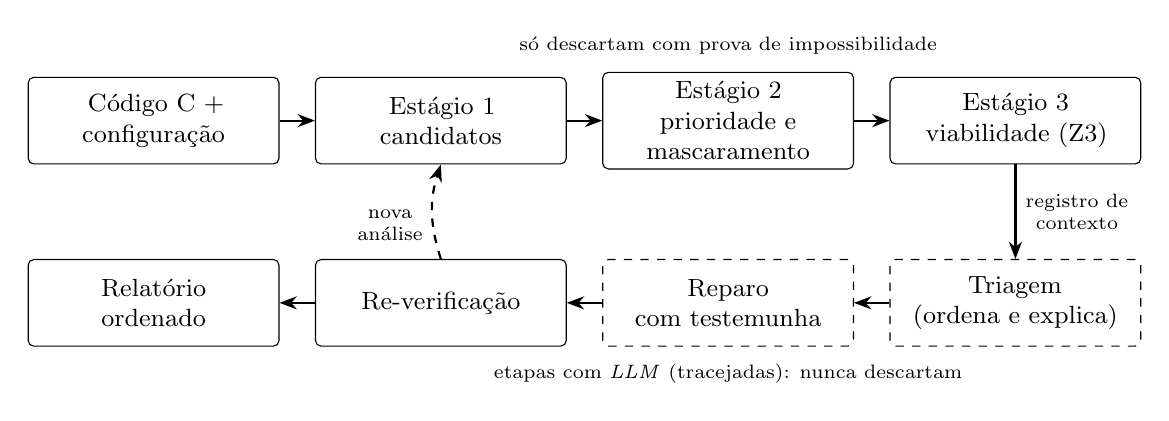
\begin{tikzpicture}[
      node distance=5mm and 4.5mm,
      etapa/.style={draw=black, rounded corners=2pt, align=center,
        minimum height=11mm, text width=29.5mm, font=\small, fill=white},
      llm/.style={etapa, dashed},
      seta/.style={-{Stealth[length=2.2mm]}, thick, color=black},
      nota/.style={font=\scriptsize, color=black, align=center}]
    \node[etapa] (cfg) {Código C +\\configuração};
    \node[etapa, right=of cfg] (e1) {Estágio 1\\candidatos};
    \node[etapa, right=of e1] (e2) {Estágio 2\\prioridade e\\mascaramento};
    \node[etapa, right=of e2] (e3) {Estágio 3\\viabilidade (Z3)};
    \node[llm, below=12mm of e3] (tri) {Triagem\\(ordena e explica)};
    \node[llm, left=of tri] (rep) {Reparo\\com testemunha};
    \node[etapa, left=of rep] (rev) {Re-verificação};
    \node[etapa, left=of rev] (rel) {Relatório\\ordenado};
    \draw[seta] (cfg) -- (e1);
    \draw[seta] (e1) -- (e2);
    \draw[seta] (e2) -- (e3);
    \draw[seta] (e3) -- node[right, nota] {registro de\\contexto} (tri);
    \draw[seta] (tri) -- (rep);
    \draw[seta] (rep) -- (rev);
    \draw[seta] (rev) -- (rel);
    \draw[seta, dashed] (rev.north) to[bend left=18] node[left, nota, pos=0.35] {nova\\análise} (e1.south);
    \node[nota, above=1mm of e2] {só descartam com prova de impossibilidade};
    \node[nota, below=1mm of rep] {etapas com \llm\ (tracejadas): nunca descartam};
  \end{tikzpicture}
  \fonte{Elaborada pelos autores.}
\end{figure}

\section{Princípio de projeto}
\label{sec:principio}

Uma única regra orienta a ferramenta: um solver pode descartar um
candidato; o \llm, não. Um resultado \textit{UNSAT} do solver é uma prova de
que a intercalação é impossível; o julgamento de um modelo de linguagem não é.
Por isso a etapa de triagem ordena, explica e agrupa os candidatos, e o
relatório final mantém todos eles.

Essa regra não é apenas prudência. A literatura mede o efeito das duas
políticas no mesmo ponto de integração: filtros com \llm\ que descartam
candidatos perdem de 6 a 25 pontos de recall \cite{reducing-fp,adataint},
enquanto a política conservadora do LLift chega a recall de 1,00
\cite{llift}. A consequência para a avaliação é que a métrica principal não é a
precisão, mas o recall, que precisa ser de 100\%, acompanhado do
\textit{Inspection Ratio}.

\section{Entrada e configuração}
\label{sec:entrada}

A ferramenta aceita um único arquivo C ou um projeto com vários arquivos. No
segundo caso, cada arquivo é compilado separadamente para a representação
intermediária do LLVM e os resultados são ligados num só módulo com
\texttt{llvm-link}. Ligar a representação intermediária, em vez de concatenar
o código-fonte, preserva a origem de cada instrução (arquivo e linha),
resolve símbolos \texttt{static} homônimos e respeita as definições de
pré-processador de cada arquivo. A compilação usa \texttt{-g}, para manter as
informações de depuração, e \texttt{-O0}, para que nenhum acesso à memória seja
eliminado por otimização.

O modelo de interrupções é dado por um arquivo de configuração escrito
à mão, que nomeia os pontos de entrada de cada fluxo, suas prioridades e as
primitivas de mascaramento da plataforma. A alternativa de inferir esse modelo
com um \llm, como \citeonline{iris} fazem com especificações de bibliotecas, foi
considerada e rejeitada: as primitivas de mascaramento formam um conjunto
fechado por plataforma, os dois benchmarks já fornecem a configuração, e
encontrar os pontos de entrada, a parte crítica para o recall, é uma busca
textual pela API de registro de interrupções, não um julgamento. O arquivo de
configuração também limita o custo: a análise percorre apenas o código
alcançável a partir dos fluxos declarados, e não o repositório inteiro.

\section{Etapa estática}
\label{sec:etapa-estatica}

\subsection{Estágio 1: candidatos}

O primeiro estágio segue o desenho de \citeonline{intrace}, que ignora
deliberadamente condições de desvio e estado das interrupções para não perder
nada. Ele resolve quatro subproblemas:

\begin{enumerate}
  \item Identificar os fluxos. Cada ponto de entrada do arquivo de
    configuração é a raiz de uma análise de alcançabilidade. Um fluxo não
    declarado não contribui com acessos, e todo defeito que dependa dele
    desaparece sem aviso; por isso esta é a primeira premissa da ferramenta.
  \item Identificar as posições compartilhadas. Uma posição é
    compartilhada quando dois ou mais fluxos a alcançam, segundo uma análise de
    ponteiros do tipo \textit{may}. Não basta considerar variáveis globais: uma
    variável local cujo endereço é guardado em ponteiros globais também pode ser
    compartilhada.
  \item Enumerar os acessos. Para cada fluxo, percorrem-se as funções
    alcançáveis e registram-se as leituras e escritas às posições
    compartilhadas, com o fluxo, o tipo de acesso, a função, o caminho de
    chamadas, a linha do código-fonte e os laços que envolvem o acesso.
  \item Derivar os candidatos. Pares e triplas são derivados
    separadamente do mesmo conjunto de acessos, pela razão discutida na
    Seção~\ref{sec:defeitos}. As triplas se restringem aos quatro padrões não
    serializáveis da Tabela~\ref{tab:padroes}.
\end{enumerate}

Um detalhe sobre laços é decisivo para o recall. Um único acesso no código-fonte,
dentro de um laço que pode repetir, corresponde a vários acessos em execução;
por isso a mesma instrução pode ser $A_1$ e $A_2$ de uma tripla. O mesmo vale
para uma função chamada mais de uma vez pelo mesmo fluxo. O Racebench anota
defeitos exatamente com essa forma.

\subsection{Estágio 2: prioridade e mascaramento}

O segundo estágio descarta candidatos cujos fluxos comprovadamente não podem se
sobrepor. Um fluxo só é interrompido por outro de prioridade estritamente
maior, com a convenção de que número maior é prioridade maior. Fluxos de mesma
prioridade são tratados como capazes de se interromper mutuamente, pois nenhum
dos modelos formais da literatura cobre esse caso e essa é a leitura que não
perde defeitos.

O mascaramento é calculado por uma análise de fluxo de dados que determina, em
cada ponto do programa, quais interrupções estão desabilitadas. Uma interrupção
só é considerada mascarada durante o intervalo $[A_1, A_2]$ de uma tripla se
(a) estiver mascarada em todo ponto de todo caminho de $A_1$ a $A_2$ no fluxo
local, e (b) nenhum fluxo que possa executar dentro desse intervalo a reabilitar.
A segunda condição é a que evita perder o defeito do caso
\texttt{svp\_simple\_001\_001} descrito na Seção~\ref{sec:interrupcoes}. Escritas
em registradores não reconhecidas nunca contam como mascaramento.

Nenhum modelo de periodicidade é assumido: o Racebench declara que uma
interrupção pode ocorrer em qualquer ponto habilitado, qualquer número de
vezes. Para pares, a pergunta é se $B$ pode executar no \textit{instante} de
$A$; para triplas, se pode executar em algum ponto do \textit{intervalo}
$[A_1, A_2]$. As duas perguntas são respondidas separadamente.

\subsection{Estágio 3: viabilidade com Z3}

O terceiro estágio aplica a análise de viabilidade de caminho de
\citeonline{intrace} com o solver Z3. Como o estágio 2, só descarta um candidato com prova, isto é, com resultado \textit{UNSAT}.
O resultado tem quatro valores (\textit{UNSAT}, \textit{SAT}, \textit{inconclusivo} e \textit{não executado}), e um resultado inconclusivo
(por limite de tempo ou construção não suportada) nunca é tratado como decidido:
o candidato segue para a triagem, com a informação de até onde o solver chegou.

A posição desse estágio antes do \llm\ é fixa por três razões: é um filtro correto, que só descarta com prova; reduz fortemente o volume (no IntRace, cerca de 208
candidatos por programa caem para cerca de 95 após o segundo estágio, e a
eliminação de 86,2\% relatada para o terceiro deixaria cerca de 13 \cite{intrace}), o que torna a triagem por \llm\ economicamente viável; e reproduz a arquitetura do LLift, em que o \llm\ recebe
apenas os casos que a execução simbólica não conseguiu decidir \cite{llift}.

\section{O registro de contexto}
\label{sec:registro}

Para cada candidato que sobrevive à etapa estática, a ferramenta emite um
registro de contexto: um documento JSON com as evidências necessárias
para julgá-lo. \citeonline{llift} atribuem 5 de seus 13 falsos positivos a
lacunas no relatório entregue pelo analisador ao modelo, o que justifica tratar
esse registro como um produto de primeira classe da análise, e não como um
subproduto. A Tabela~\ref{tab:registro} resume seus campos.

\begin{table}[htb]
  \centering
  \caption{Campos do registro de contexto}
  \label{tab:registro}
  \begin{tabular}{@{}lL{11cm}@{}}
    \toprule
    Campo & Conteúdo \\
    \midrule
    classe & par (\textit{data race}) ou tripla (violação de atomicidade) \\
    variável & nome, tipo, se é \texttt{volatile}, local da declaração \\
    acessos & para cada um: leitura ou escrita, linha, função e fluxo \\
    fluxos & ponto de entrada, prioridade e como o fluxo foi identificado \\
    caminhos & sequência de chamadas do ponto de entrada até cada acesso \\
    mascaramento & estado de cada interrupção em cada acesso e no intervalo \\
    laços & laços que envolvem cada acesso; se $A_1$ e $A_2$ são a mesma instrução \\
    código & corpo completo das funções que contêm os acessos \\
    solver & veredicto do Z3 e, se inconclusivo, o motivo \\
    proveniência & quais fatos foram provados, quais vêm da configuração, quais são desconhecidos \\
    \bottomrule
  \end{tabular}
  \fonte{Elaborada pelos autores.}
\end{table}

O registro não traz um fatiamento de programa pré-calculado. Um
fatiamento sobre uma variável global tende a abarcar quase todo o programa, e um
fatiamento incompleto leva o modelo a declarar, com confiança, que um defeito
real é impossível. Em vez disso, o registro traz as camadas sempre úteis, e o
modelo pede o que falta. O campo de proveniência serve ao mesmo propósito:
evidência parcial é marcada como parcial.

\section{Etapa com modelo de linguagem}
\label{sec:etapa-llm}

\subsection{Triagem: duas perguntas, quatro grupos}

O modelo nunca escolhe diretamente onde o candidato fica. Ele responde a duas
perguntas estreitas: a intercalação pode acontecer? (viabilidade) e,
se puder, ela causa dano? (nocividade). Separar as perguntas evita que
``benigno'' se transforme silenciosamente em ``impossível''. O grupo do
candidato é derivado das duas respostas por uma tabela fixa
(Tabela~\ref{tab:grupos}), na qual qualquer dúvida sobe o candidato na fila.

\begin{table}[htb]
  \centering
  \caption{Derivação do grupo de cada candidato, em ordem de leitura}
  \label{tab:grupos}
  \begin{tabular}{@{}cL{3.6cm}L{6.0cm}L{3.4cm}@{}}
    \toprule
    Ordem & Grupo & Viabilidade & Nocividade \\
    \midrule
    1 & provavelmente real & possível & nociva \\
    2 & incerto & incerta, ou possível com nocividade incerta & qualquer \\
    3 & provavelmente benigno & possível & benigna \\
    4 & provavelmente inviável & impossível, com o elemento que impede & não perguntada \\
    \bottomrule
  \end{tabular}
  \fonte{Elaborada pelos autores.}
\end{table}

Todos os grupos aparecem no relatório. O grupo só determina a posição de leitura,
e é essa ordem que o \textit{Inspection Ratio} avalia.

\subsection{Desenho do \textit{prompt}}

O desenho segue os quatro componentes de \citeonline{llift}, adaptados ao
domínio:

\begin{itemize}
  \item Regras do domínio por exemplos. O conhecimento prévio do modelo
    vem sobretudo de \textit{threads} e o leva a procurar travas e relações
    \textit{happens-before}. O \textit{prompt} ensina uma tabela de padrões de
    interrupção com seus veredictos: uma seção crítica cobrindo todo o intervalo
    torna a tripla inviável; duas seções separadas deixam uma lacuna em que a
    \isr\ cabe; prioridade estritamente menor impede a preempção, e prioridade
    igual não; a mesma instrução num laço pode formar uma tripla consigo mesma.
  \item Pedidos progressivos de contexto. O modelo pode pedir, num
    formato fixo, a definição de uma função, o corpo de uma \isr, o estado de
    mascaramento numa linha ou a expansão de uma macro. O registro dos pedidos
    mede, na prática, que contexto o registro deveria trazer.
  \item Decomposição da tarefa. Viabilidade e nocividade são perguntadas
    em conversas separadas.
  \item Autovalidação enviesada para o recall. Antes de responder, o
    modelo confere regras como: mascaramento desconhecido conta como
    habilitado; uma função cuja definição não foi obtida pode acessar a
    variável; ``incerto'' é sempre uma resposta segura.
\end{itemize}

O modelo raciocina antes de dar o veredicto, e a resposta final é uma saída
estruturada com a explicação antes do veredicto, como recomendam
\citeonline{iris}. O código analisado é delimitado e declarado como
dado, nunca instrução: um comentário no código que tente convencer o
modelo a ignorar um defeito não pode ter efeito \cite{sastgenius}.

A etapa é construída de forma independente do provedor do modelo. Isso permite
manter o \textit{prompt} fixo e trocar o modelo, e assim verificar neste domínio a
afirmação de \citeonline{llift} de que a arquitetura do \textit{prompt} pesa mais
que a escolha do modelo.

\subsection{Reparo com testemunha}

Para cada candidato, o modelo pode propor uma correção no vocabulário
específico de interrupções enumerado por \citeonline{sdracer}: desabilitar e
reabilitar a interrupção em volta do acesso, estender uma seção crítica
existente ou fundir seções adjacentes. O escopo depende da classe do defeito:
um \textit{data race} se corrige protegendo um acesso; uma violação de
atomicidade, tornando todo o intervalo $[A_1, A_2]$ atômico.

Inspirada na validação por \textit{exploits} de \citeonline{sastgenius}, toda
proposta de correção exige uma testemunha: qual \isr\ dispara, em que
ponto, em que ordem ocorrem os acessos e que estado resulta diferente de
qualquer execução em série. A testemunha é conferida mecanicamente contra o
registro de contexto antes de a correção ser aceita.

\section{Re-verificação}
\label{sec:reverificacao}

Uma correção é verificada em duas etapas, que falham em direções opostas.
Primeiro, a própria análise estática é executada de novo sobre o programa
corrigido. Como seus filtros só descartam com prova, o desaparecimento do
candidato é uma certificação, sob as premissas declaradas, de que o defeito
sumiu; e a nova análise completa é a única forma de detectar
regressões, como uma seção crítica estendida que cria outro defeito.
Se o candidato persistir, o resultado é inconclusivo, pois uma análise
superaproximada pode continuar reportando um defeito já corrigido. Segundo, os
casos inconclusivos são resolvidos por um verificador limitado (o CBMC \cite{cbmc} ou o próprio BMC4AV, cujo código-fonte está disponível), codificando a violação como uma asserção. Por fim, como observado por
\citeonline{sdracer}, verifica-se se a correção alterou o fluxo de controle ou
a latência, que em código de interrupção é uma propriedade de correção.

\section{Interface}
\label{sec:interface}

A ferramenta é pensada para ser operada por um painel, e não apenas por linha
de comando: configurar um programa, executar a análise, ler cada candidato ao
lado do código-fonte e aceitar ou rejeitar uma correção. A literatura compete,
na prática, em automação: cada ferramenta nova ataca o trabalho manual exigido pela anterior \cite{intrace,nichecker,bmc4av}. Por isso, a usabilidade é tratada aqui como parte da contribuição.

\section{Contratos entre as etapas}
\label{sec:contratos}

Para que as duas frentes possam avançar em paralelo, as interfaces entre elas
são definidas como esquemas JSON, com exemplos (Tabela~\ref{tab:contratos}).
\ifparcial\else O Apêndice~\ref{ap:contratos} os detalha.\fi

\begin{table}[htb]
  \centering
  \caption{Contratos entre as partes da ferramenta}
  \label{tab:contratos}
  \begin{tabular}{@{}llll@{}}
    \toprule
    & Contrato & Produz & Consome \\
    \midrule
    C1 & arquivo de configuração (modelo de interrupções) & frente A & frentes A e C \\
    C2 & registro de contexto de cada candidato & frente A & frentes B e C \\
    C3 & organização de uma execução em disco & frente A & frentes B e C \\
    C4 & pedidos de contexto e respostas & frente B & frente A \\
    \bottomrule
  \end{tabular}
  \fonte{Elaborada pelos autores.}
\end{table}

\section{Premissas e ameaças ao recall}
\label{sec:premissas}

A afirmação de que a ferramenta não perde defeitos vale em relação a uma lista
explícita de premissas, mantida junto com o código. As principais são:

\begin{itemize}
  \item o arquivo de configuração nomeia todos os fluxos; um tratador não
    declarado é invisível, e esta é a maior ameaça ao recall;
  \item uma chamada indireta cujos alvos não se resolvem pode chamar qualquer
    função de assinatura compatível cujo endereço foi tomado;
  \item posições compartilhadas são identificadas por análise \textit{may}, e a
    correção da análise de ponteiros do SVF é herdada, não reverificada;
  \item uma função sem corpo no programa pode ler e escrever qualquer variável
    global;
  \item fluxos de mesma prioridade podem se interromper, e o aninhamento é
    permitido;
  \item uma interrupção só está mascarada se estiver mascarada em todos os
    caminhos, e nenhum outro fluxo a reabilitar no intervalo;
  \item só uma prova descarta um candidato; o resultado inconclusivo do solver e
    o julgamento do \llm\ nunca descartam.
\end{itemize}

Uma premissa é deliberadamente não conservadora: por padrão, uma \isr\
não interrompe a si mesma. O Racebench não exclui a reentrância e a literatura
diverge sobre ela; a escolha fica registrada para revisão antes de qualquer
afirmação final de recall.

\chapter{Metodologia de avaliação}
\label{cap:metodologia}

% wiki: LLM Stage Design (Testing and evaluation), concepts/Precision Metrics,
% benchmarks/Racebench; project-src/docs/evaluation-protocol.md

Este capítulo define como a ferramenta será avaliada: as perguntas de pesquisa,
o gabarito contra o qual se mede, as métricas, o protocolo experimental e as
ameaças à validade.

\section{Perguntas de pesquisa}
\label{sec:qp}

\begin{description}
  \item[QP1] A etapa estática encontra todos os defeitos anotados no Racebench,
    isto é, atinge recall de 100\%?
  \item[QP2] A triagem por \llm\ reduz o esforço de revisão sem que nenhum
    defeito real seja classificado como inviável?
  \item[QP3] Qual a contribuição de cada técnica de \textit{prompt}? Essa pergunta
    é respondida por uma ablação no formato de \citeonline{llift}.
  \item[QP4] O \llm\ propõe correções corretas para os defeitos encontrados?
\end{description}

\section{Benchmarks e gabarito}
\label{sec:benchmarks}

\subsection{Unidade de contagem}

Toda taxa de recall divide por um número de defeitos, e a literatura usa números
diferentes para os mesmos programas sem dizer por quê
(Seção~\ref{sec:rel-comparacao}). Este trabalho adota explicitamente
uma tripla anotada como um defeito. Medidas sobre os 31 casos simples
do Racebench, as unidades possíveis dão resultados bem diferentes
(Tabela~\ref{tab:unidades}).

\begin{table}[htb]
  \centering
  \caption{Contagem do gabarito do Racebench conforme a unidade}
  \label{tab:unidades}
  \begin{tabular}{@{}lcc@{}}
    \toprule
    Unidade & Defeitos & Armadilhas \\
    \midrule
    por instância de tripla & 48 & 38 \\
    por par (caso, variável) & 33 & 29 \\
    por caso & 31 & 31 \\
    \bottomrule
  \end{tabular}
  \fonte{Elaborada pelos autores a partir das anotações de \citeonline{racebench}.}
\end{table}

A unidade por instância é a mais fina, e portanto a mais difícil de inflar; é a
usada pelo BMC4AV, o que preserva a comparação; e as unidades mais grossas
escondem estrutura: um mesmo caso chega a ter quatro defeitos distintos
numa só variável.

\subsection{Leitura e correção do gabarito}

As anotações do Racebench usam ao menos quatro gramáticas incompatíveis e contêm
erros: um leitor estrito encontra apenas 28 defeitos, sem acusar erro. Por isso
o leitor de gabarito precisa tolerar as variações, e sua contagem é validada
contra uma contagem manual dos casos mais difíceis antes de qualquer medição.

Doze anotações são corrigidas antes da comparação, por uma errata em que cada
correção traz sua evidência: seis números de linha (cinco deles num único caso cujas anotações apontam para linhas sem nenhum acesso) e seis tipos de acesso trocados.
Nenhuma correção altera as contagens. Sem elas, uma comparação exata com o texto
distribuído daria recall zero para um defeito que a ferramenta encontra na linha
certa.

\subsection{Regra de casamento}

Um candidato reportado corresponde a uma tripla anotada quando está no
mesmo programa, trata da mesma posição de memória e tem as mesmas linhas
ordenadas $(A_1, B, A_2)$ que a anotação corrigida. Três escolhas são
deliberadas:

\begin{itemize}
  \item o tipo de acesso não precisa coincidir, porque as linhas já distinguem
    todas as 86 anotações sem colisão e 20 acessos anotados estão em linhas que
    leem e escrevem a variável;
  \item o nome da variável é comparado depois de resolver apelidos, pois 12
    anotações nomeiam a posição por um ponteiro, um elemento de vetor ou um campo de estrutura;
  \item o recall é medido apenas sobre triplas; os pares recebem uma medida
    própria de cobertura, publicada ao lado.
\end{itemize}

\subsection{Conjunto de triagem}

A etapa com \llm\ é desenvolvida e medida, até a integração com a etapa
estática, sobre 20 registros de contexto montados à mão a partir do
Racebench: 10 defeitos anotados e 10 armadilhas, organizados de modo a formar
seis pares adversariais, isto é, um defeito e uma armadilha que diferem em um
único detalhe, como o estado de mascaramento. Os pares existem para que o modelo não
acerte pela aparência do código. Um caso cujas anotações descrevem uma versão
diferente do programa distribuído foi excluído do conjunto.

\subsection{Suíte de programas reais}

A suíte de 18 programas (Seção~\ref{sec:rel-benchmarks}) é usada na etapa final.
Seu gabarito registra, por variável, 45 violações verdadeiras e 14 falsas, o
que também a torna um conjunto de triagem.

\section{Métricas}
\label{sec:metricas}

\begin{description}
  \item[Portão de recall] Todos os defeitos anotados precisam chegar ao relatório
    e nenhum pode ser classificado como provavelmente inviável. Uma falha aqui
    é um defeito de projeto, não um ajuste.
  \item[Rejeição de armadilhas] Fração das armadilhas classificadas nos grupos
    baixos. É a medida de precisão da triagem e, ao contrário da precisão, não
    melhora descartando candidatos.
  \item[\textit{Inspection Ratio}] Fração da lista ordenada que um revisor
    precisa ler até encontrar todos os defeitos \cite{reducing-fp}. Empates de
    grupo e confiança são resolvidos pelo pior caso, colocando o defeito real por
    último.
  \item[Consistência] Concordância entre execuções repetidas do mesmo candidato.
    \citeonline{llift} mostram que a decomposição e a autovalidação a melhoram
    independentemente da acurácia.
  \item[Taxas de reparo] Taxa sintática (um analisador sintático aceita a correção) e taxa
    lógica (a correção equivale a uma escrita à mão), como em
    \citeonline{skipanalyzer}, seguidas da re-verificação.
\end{description}

No Racebench, apenas a viabilidade entra nessas métricas. O gabarito anota
fatos do programa (a intercalação existe), e muitos de seus defeitos leem
a variável compartilhada para uma variável local que nunca é usada. Um modelo
que classifica esses casos como benignos está raciocinando corretamente sobre o
código, e pontuar essa resposta contra o gabarito puniria o acerto. A pergunta
de nocividade continua sendo feita e registrada, e é avaliada na suíte de
programas reais, em que o código tem efeito observável.

\section{Protocolo experimental}
\label{sec:protocolo}

\subsection{Ablação}

A ablação acrescenta um componente de \textit{prompt} por linha, sempre sobre os
mesmos candidatos: \textit{prompt} simples; mais regras do domínio; mais pedidos
progressivos de contexto; mais decomposição da tarefa; mais autovalidação. Como
os pedidos de contexto só trazem informação nova quando respondidos a partir do
código real, a linha correspondente é medida depois da integração com o
resolvedor da etapa estática.

Na ablação do LLift, o \textit{prompt} simples já perdia a maioria dos defeitos,
e o recall era a variável que se movia. Se, neste domínio, o recall já partir de
100\%, as variáveis dependentes da ablação passam a ser a rejeição de armadilhas
e o \textit{Inspection Ratio}.

\subsection{Registro e reprodutibilidade}

Todo número é registrado com o modelo, a data e a configuração de
\textit{prompt} que o produziram, pois as comparações de modelos da literatura
envelhecem rapidamente. As respostas do modelo são guardadas em cache,
indexadas pelo candidato, pela configuração e pelo modelo, de modo que uma
mesma medição possa ser recalculada sem nova chamada. O custo em
\textit{tokens} e em tempo é medido por candidato. Uma linha da ablação só é
considerada medida se cobrir todos os candidatos previstos.

\section{Ameaças à validade}
\label{sec:ameacas}

\begin{itemize}
  \item Amostra pequena. Vinte candidatos e uma amostra por candidato
    tornam diferenças de um ou dois candidatos indistinguíveis de ruído; a
    medição de consistência com várias amostras é o que permite afirmar uma
    diferença.
  \item Ajuste sobre o conjunto de teste. Quando o \textit{prompt} é
    corrigido depois de observar erros nos mesmos 20 casos, o número seguinte é
    otimista. Por isso as versões anteriores e posteriores são reportadas lado a
    lado.
  \item Gabarito com erros conhecidos. A errata corrige o que pode ser
    verificado no código; o rótulo de um caso cujas anotações descrevem outra
    versão do programa não pode ser corrigido sem decidir de novo o gabarito.
  \item População diferente após a integração. Com a etapa estática
    completa, o \llm\ recebe apenas o que o solver não decidiu, que são os casos
    mais difíceis; os números obtidos sobre os 20 registros montados à mão não
    se transferem automaticamente.
  \item Benchmarks de arquivo único. Todos os programas avaliados são um
    único arquivo; a entrada com vários arquivos é uma capacidade da ferramenta
    exercida fora do gabarito.
  \item Premissas não conservadoras. A exclusão de reentrância
    (Seção~\ref{sec:premissas}) é uma perda potencial de recall registrada, não
    medida.
\end{itemize}

\chapter{Implementação}
\label{cap:implementacao}

% Só na monografia completa (final.tex).

\section{Processo e ferramentas}
\pendente{LLVM, SVF, Z3, Python; o plano de trabalho da parcial vira esta seção.}

\section{Etapa estática}
\pendente{}

\section{Etapa de LLM}
\pendente{Harness independente de provedor, cache, pontuação.}

\section{Reparo e re-verificação}
\pendente{}

\chapter{Avaliação}
\label{cap:avaliacao}

% Só na monografia completa (final.tex).

\section{QP1: recall da análise estática}
\pendente{}

\section{QP2 e QP3: ablação da triagem}
\pendente{Tabela do M3; versões 1 e 2 das regras de domínio lado a lado.}

\section{QP4: reparo}
\pendente{}

\section{Suíte real}
\pendente{}

\section{Custo}
\pendente{}

\section{Discussão}
\pendente{}

\chapter{Conclusão}
\label{cap:conclusao}

% Só na monografia completa (final.tex).

\section{Contribuições}
\pendente{}

\section{Limitações}
\pendente{}

\section{Trabalhos futuros}
\pendente{}


\postextual

\bibliography{referencias}

\begin{apendicesenv}
\partapendices
\chapter{Contratos entre as etapas}
\label{ap:contratos}

% Fonte: project-src/contracts/README.md e os esquemas JSON.

Os quatro contratos da Tabela~\ref{tab:contratos} foram escritos como esquemas
JSON, com exemplos, e não como texto. Cada documento carrega uma versão; um
consumidor aceita qualquer documento com a mesma versão principal e ignora
campos desconhecidos, e mudanças incompatíveis exigem nova versão principal.

\section{C1: arquivo de configuração}

Descreve o modelo de interrupções de um programa: os fluxos, com ponto de
entrada e prioridade; as primitivas de mascaramento; o tratamento de funções
externas; e as opções semânticas, como a preempção entre fluxos de mesma
prioridade e a reentrância. As opções que afetam o recall trazem o valor
conservador como padrão.

\section{C2: registro de contexto}

Um documento por candidato, com os campos da Tabela~\ref{tab:registro}. Cinco
decisões de projeto estão codificadas na própria estrutura, para que não possam
ser revertidas sem que alguém perceba:

\begin{enumerate}
  \item o mascaramento tem três valores (desabilitado, habilitado e desconhecido), e não existe um campo booleano ``mascarado'';
  \item o estado de mascaramento num ponto e ao longo de um intervalo são campos
    distintos, pois responder um e inferir o outro perde defeitos;
  \item o veredicto do solver tem quatro valores, e o inconclusivo exige um
    motivo;
  \item a proveniência dos fatos é obrigatória;
  \item não existe campo de fatiamento: o contexto adicional é obtido pelo
    contrato C4.
\end{enumerate}

Cada registro traz ainda uma impressão digital que depende apenas do programa,
da classe, da variável e das posições dos acessos, usada como chave do cache de
respostas do modelo.

\section{C3: organização de uma execução}

Define os diretórios e arquivos de uma execução da ferramenta: um manifesto com
a configuração, as versões e as decisões de avaliação usadas; os candidatos de
cada estágio; e o histórico das conversas com o modelo. Uma execução em que algum
candidato não tenha nem registro de contexto nem prova de impossibilidade é
rejeitada pela verificação do próprio formato.

\section{C4: pedidos de contexto}

Define o que o modelo pode pedir e como a resposta volta. Os tipos de pedido
incluem a definição de uma função, o corpo de uma \isr, o estado de mascaramento
numa linha, a expansão de uma macro, todos os acessos a uma variável e todos os
caminhos de chamada até uma função. Toda resposta traz um estado (resolvido, não encontrado, não suportado, truncado, ambíguo ou recusado) e, quando o
pedido não pôde ser atendido, a regra de recall que se aplica. Uma definição
não encontrada, por exemplo, deve ser tratada como uma função que pode acessar
a variável; uma resposta vazia nunca pode ser lida como ``não há nada''.

\end{apendicesenv}

\end{document}
